% Gabarit pandoc des corrigés publiés (brut et guidé). Contenu sans marque ni nom de site.
% Compilation : lualatex (latexmk -lualatex).
% Le Markdown reste la source unique : ne pas éditer ce fichier .tex à la main.
\documentclass[11pt,a4paper]{article}

% --- Moteur, polices (Latin Modern) et langue ---------------------------------
\usepackage{iftex}
\ifLuaTeX\else\errmessage{Ce document se compile avec lualatex}\fi
\usepackage{amsmath,amssymb,mathtools}
\usepackage{fontspec}
% mathrm=sym : \mathrm prend ses glyphes dans la police mathématique (ℓ, μ, Ω), comme KaTeX.
\usepackage[math-style=TeX,bold-style=TeX,mathrm=sym]{unicode-math}
% Repli pour les glyphes absents de Latin Modern (indices et exposants Unicode,
% flèches, filets des schémas en texte, symboles) : DejaVu, puis Latin Modern Math
% (ℓ, lettres mathématiques Unicode des légendes).
\directlua{
  luaotfload.add_fallback("repliTexte", {"DejaVuSerif:mode=harf;", "DejaVuSans:mode=harf;", "file:latinmodern-math.otf:mode=harf;"})
  luaotfload.add_fallback("repliMono", {"DejaVuSansMono:mode=harf;", "DejaVuSans:mode=harf;", "file:latinmodern-math.otf:mode=harf;"})
}
\setmainfont{Latin Modern Roman}[RawFeature={fallback=repliTexte}]
\setsansfont{Latin Modern Sans}[RawFeature={fallback=repliTexte}]
\setmonofont{Latin Modern Mono}[RawFeature={fallback=repliMono}]
\setmathfont{Latin Modern Math}
\usepackage[french]{babel}
\frenchsetup{SmallCapsFigTabCaptions=false}

% --- Mise en page --------------------------------------------------------------
\usepackage[a4paper,margin=2.2cm,headheight=14pt,footskip=1.2cm]{geometry}
\usepackage{microtype}
\setlength{\emergencystretch}{4em}
\tolerance=1500
\setlength{\parindent}{0pt}
\setlength{\parskip}{0.55\baselineskip plus 2pt minus 1pt}
\usepackage{xcolor}
% Gris nommés : babel-french rend « ! » actif dans le document.
\definecolor{gris2}{gray}{0.98}
\definecolor{gris3}{gray}{0.97}
\definecolor{gris5}{gray}{0.95}
\definecolor{gris35}{gray}{0.65}
\definecolor{gris40}{gray}{0.60}
\definecolor{gris45}{gray}{0.55}
\definecolor{gris50}{gray}{0.50}
\definecolor{gris55}{gray}{0.45}
\definecolor{gris60}{gray}{0.40}
\definecolor{gris65}{gray}{0.35}
\definecolor{gris70}{gray}{0.30}
\definecolor{gris80}{gray}{0.20}
\definecolor{gris85}{gray}{0.15}
\usepackage{graphicx}
\usepackage{float}
\usepackage{caption}
\captionsetup{font=small,labelformat=empty,justification=centering}
\usepackage{booktabs,longtable,array,multirow,calc}
\usepackage{siunitx}
\sisetup{locale=FR}
\usepackage[version=4]{mhchem}
\usepackage{listings}
\usepackage{fancyhdr}
\usepackage{lastpage}
\usepackage[most]{tcolorbox}
\usepackage{enumitem}
\setlist{nosep,leftmargin=*,topsep=2pt}
\usepackage[hidelinks,unicode]{hyperref}
\usepackage{bookmark}
\hypersetup{pdftitle={Centrale-Supélec PSI — Mathématiques 2 2026},pdfauthor={Rédigé par IA},pdfcreator={LaTeX},pdfsubject={Corrigé brut}}
\usepackage{xurl}

% --- Pandoc : listes, tableaux, figures ----------------------------------------
\providecommand{\passthrough}[1]{#1}
\providecommand{\tightlist}{\setlength{\itemsep}{0pt}\setlength{\parskip}{0pt}}

\makeatletter
\def\maxwidth{\ifdim\Gin@nat@width>\linewidth\linewidth\else\Gin@nat@width\fi}
\def\maxheight{\ifdim\Gin@nat@height>0.55\textheight 0.55\textheight\else\Gin@nat@height\fi}
\makeatother
\setkeys{Gin}{width=\maxwidth,height=\maxheight,keepaspectratio}
\setcounter{secnumdepth}{-\maxdimen}
\providecommand{\pandocbounded}[1]{#1}

% --- Code (listings) -----------------------------------------------------------
\lstset{
  basicstyle=\ttfamily\small,
  columns=fullflexible,
  keepspaces=true,
  breaklines=true,
  breakatwhitespace=false,
  postbreak=\mbox{\textcolor{gris50}{$\hookrightarrow$}\space},
  frame=single,
  rulecolor=\color{gris35},
  framesep=4pt,
  xleftmargin=5pt,xrightmargin=5pt,
  backgroundcolor=\color{gris3},
  keywordstyle=\bfseries,
  commentstyle=\color{gris65},
  stringstyle=\color{gris80},
  showstringspaces=false,
  tabsize=4,
  extendedchars=true,
  aboveskip=6pt,belowskip=6pt,
}

% --- Macros des corrigés (KaTeX ↔ LaTeX) ---------------------------------------
% Les corrigés sont écrits pour KaTeX : on définit ici ce que KaTeX connaît et
% que LaTeX n'a pas, sans jamais retoucher le Markdown.
\providecommand{\R}{\mathbb{R}}
\providecommand{\N}{\mathbb{N}}
\providecommand{\Z}{\mathbb{Z}}
\providecommand{\Q}{\mathbb{Q}}
\providecommand{\C}{\mathbb{C}}
\providecommand{\dd}{\mathrm{d}}
\providecommand{\llbracket}{\lBrack}
\providecommand{\rrbracket}{\rBrack}
\providecommand{\lBrace}{\lbrace}
\providecommand{\rBrace}{\rbrace}
\providecommand{\Box}{\square}
\providecommand{\Diamond}{\lozenge}
\providecommand{\varnothing}{\emptyset}
\providecommand{\argmax}{\operatorname*{arg\,max}}
\providecommand{\argmin}{\operatorname*{arg\,min}}
\renewcommand{\leq}{\leqslant}
\renewcommand{\geq}{\geqslant}

% Équation hors texte : réduite à la largeur de la ligne si elle déborde.
\newsavebox{\boiteequation}
\newcommand{\equationajustee}[1]{%
  \sbox{\boiteequation}{$\displaystyle #1$}%
  \ifdim\wd\boiteequation>\linewidth
    \[\resizebox{\linewidth}{!}{\usebox{\boiteequation}}\]%
  \else
    \[#1\]%
  \fi}

% --- Encadrés pédagogiques (sobres, lisibles en noir et blanc) -----------------
\tcbset{
  encadre/.style={
    enhanced,breakable,sharp corners,
    colback=white,colframe=gris55,
    boxrule=0.4pt,leftrule=2.2pt,
    left=6pt,right=6pt,top=3pt,bottom=3pt,
    before skip=6pt,after skip=6pt,
    fonttitle=\bfseries\small,coltitle=black,
    attach title to upper,after title={\quad},
    parbox=false,
  }
}
\newtcolorbox{indication}[1]{encadre,colframe=gris45,colback=gris2,title={Indication~#1}}
\newtcolorbox{methode}{encadre,colframe=gris70,title={Méthode}}
\newtcolorbox{piege}{encadre,colframe=gris85,boxrule=0.8pt,leftrule=2.2pt,title={Piège}}
\newtcolorbox{jury}{encadre,colframe=gris60,colback=gris5,title={Jury}}
\newtcolorbox{encadrenote}{encadre,colframe=gris40}

% --- Titres de section ---------------------------------------------------------
\usepackage{titlesec}
\titleformat{\section}{\Large\bfseries}{}{0pt}{}
\titleformat{\subsection}{\large\bfseries}{}{0pt}{}
\titleformat{\subsubsection}{\normalsize\bfseries}{}{0pt}{}
\titlespacing*{\section}{0pt}{14pt plus 4pt minus 2pt}{6pt}
\titlespacing*{\subsection}{0pt}{10pt plus 3pt minus 2pt}{4pt}
\titlespacing*{\subsubsection}{0pt}{8pt plus 2pt minus 2pt}{2pt}

% --- En-tête et pied de page ---------------------------------------------------
\pagestyle{fancy}
\fancyhf{}
\fancyhead[L]{\small\textsc{Corrigé brut} · Centrale-Supélec PSI}
\fancyhead[R]{\small Maths 2 2026}
\fancyfoot[L]{\footnotesize Corrigé rédigé par IA, non officiel}
\fancyfoot[R]{\footnotesize \thepage\,/\,\pageref*{LastPage}}
\renewcommand{\headrulewidth}{0.4pt}
\renewcommand{\footrulewidth}{0pt}
\fancypagestyle{plain}{\fancyhf{}\fancyfoot[R]{\footnotesize \thepage\,/\,\pageref*{LastPage}}\fancyfoot[L]{\footnotesize Corrigé rédigé par IA, non officiel}\renewcommand{\headrulewidth}{0pt}}

\begin{document}
\thispagestyle{plain}
\begin{center}
  {\small\scshape Corrigé brut}\par\smallskip
  {\LARGE\bfseries Centrale-Supélec PSI — Mathématiques 2 2026\par}\medskip
  {\large Centrale-Supélec · PSI · Maths 2 · 2026\par}
\end{center}
\vspace{2pt}\hrule\vspace{8pt}

\emph{Corrigé rédigé par IA, non officiel. Signalez toute erreur.}

\textbf{Polynômes de Jacobi.} Durée 4 heures, calculatrice autorisée. 42 questions.

Notations : \(\mathbb R_k[X]=\mathrm{Vect}(1,X,\dots,X^k)\) ; \(w(t)=(1-t)^\alpha(1+t)^\beta\) ; \(\alpha,\beta>-1\) sauf mention contraire.

\hypertarget{partie-a-un-produit-scalaire}{%
\section{Partie A --- Un produit scalaire}\label{partie-a-un-produit-scalaire}}

\hypertarget{q1}{%
\subsection{Q1}\label{q1}}

L'intégrale de Riemann \(\displaystyle\int_0^1\frac{dt}{t^\delta}\) converge si et seulement si \(\delta<1\), et alors

\equationajustee{\boxed{\begin{aligned}\int_0^1\frac{dt}{t^\delta}&=\Big[\frac{t^{1-\delta}}{1-\delta}\Big]_0^1\\&=\frac1{1-\delta}.\end{aligned}}}

\hypertarget{q2}{%
\subsection{Q2}\label{q2}}

Soit \(a>0\). La fonction \(t\mapsto(a-t)^{-\delta}\) est continue sur \([0,a[\). L'intégrale n'est donc impropre qu'en \(a\), et seulement si \(\delta>0\).

Le changement de variable \(u=a-t\) est une bijection de classe \(\mathcal C^1\) strictement décroissante de \(]0,a[\) sur lui-même. Les deux intégrales suivantes sont donc de même nature, et égales en cas de convergence :

\equationajustee{\int_0^a\frac{dt}{(a-t)^\delta}\quad\text{et}\quad\int_0^a\frac{du}{u^\delta}.}

Le changement de variable \(u=av\) ramène ensuite à Q1 :

\equationajustee{\int_0^a\frac{du}{u^\delta}=a^{1-\delta}\int_0^1\frac{dv}{v^\delta}.}

Par Q1 :

\equationajustee{\boxed{\begin{aligned}{}&\int_0^a\frac{dt}{(a-t)^\delta}\ \text{converge}\iff\delta<1,\\&\text{et alors elle vaut }\frac{a^{1-\delta}}{1-\delta}.\end{aligned}}}

Cas restants. Si \(a=0\), l'intégrale est nulle.

Si \(a<0\), la quantité \(a-t\) est négative sur l'intervalle d'intégration. La puissance \((a-t)^\delta\) n'est alors définie que pour \(\delta\) entier.

On trouve encore la condition \(\delta<1\). En effet, pour \(\delta\leqslant 0\), on intègre un polynôme. Pour \(\delta\geqslant1\), l'intégrale diverge en \(t=a\).

Seul le cas \(a>0\) sert dans la suite.

\hypertarget{q3}{%
\subsection{Q3}\label{q3}}

Posons \(h(t)=(1-t)^\alpha(1+t)^\beta f(t)\), continue sur \(]-1,1[\). On coupe en \(0\).

\emph{En \(1\).} La fonction \(t\mapsto(1+t)^\beta f(t)\) est continue sur le segment \([0,1]\). Elle y est donc bornée par un réel \(M_1\), et, sur \([0,1[\) :

\equationajustee{|h(t)|\leqslant M_1(1-t)^\alpha.}

On applique Q2 avec \(a=1\) et \(\delta=-\alpha\). Comme \(-\alpha<1\), l'intégrale \(\int_0^1(1-t)^\alpha dt\) converge. Par comparaison de fonctions positives, \(\int_0^1|h|\) converge.

\emph{En \(-1\).} De même, sur \(]-1,0]\) :

\equationajustee{|h(t)|\leqslant M_2(1+t)^\beta.}

Le changement de variable \(u=-t\) donne \(\int_{-1}^0(1+t)^\beta dt=\int_0^1(1-u)^\beta du\). Cette intégrale converge car \(-\beta<1\).

Donc \(h\) est intégrable sur \(]-1,1[\) : \textbf{l'intégrale \(\int_{-1}^1(1-t)^\alpha(1+t)^\beta f(t)\,dt\) converge (absolument).}

\hypertarget{q4}{%
\subsection{Q4}\label{q4}}

\emph{Bonne définition} : soient \(P,Q\in\mathbb R[X]\). Le produit \(PQ\) est continu sur \([-1,1]\), donc \(\langle P,Q\rangle\) existe par Q3.

\emph{Symétrie} : évidente. \emph{Bilinéarité} : par symétrie, la linéarité à gauche suffit ; elle découle de la linéarité de l'intégrale (toutes les intégrales en jeu convergent).

\emph{Positivité} : \(w(t)P(t)^2\geqslant0\) sur \(]-1,1[\), donc \(\langle P,P\rangle\geqslant0\).

\emph{Caractère défini} : supposons \(\langle P,P\rangle=0\). Pour tout segment \([c,d]\subset]-1,1[\), on a

\equationajustee{\begin{aligned}0&\leqslant\int_c^d wP^2\\&\leqslant\int_{-1}^1wP^2\\&=0.\end{aligned}}

La fonction \(wP^2\) est continue et positive sur le segment \([c,d]\), et d'intégrale nulle : elle y est nulle. Comme \(w>0\), \(P\) s'annule sur \([c,d]\). Il a donc une infinité de racines : \(P=0\).

\textbf{\(\langle\cdot,\cdot\rangle\) est un produit scalaire sur \(\mathbb R[X]\).}

\hypertarget{i-un-premier-exemple-alphabeta-tfrac12}{%
\subsection{\texorpdfstring{I -- Un premier exemple (\(\alpha=\beta=-\tfrac12\))}{I -- Un premier exemple (\textbackslash alpha=\textbackslash beta=-\textbackslash tfrac12)}}\label{i-un-premier-exemple-alphabeta-tfrac12}}

\hypertarget{q5}{%
\subsection{Q5}\label{q5}}

On a \(\langle1,\allowbreak X\rangle=\displaystyle\int_{-1}^1\frac{t\,dt}{\sqrt{1-t^2}}\), convergente par Q3. Une primitive sur \(]-1,1[\) est \(-\sqrt{1-t^2}\). Elle tend vers \(0\) en \(\pm1\) :

\equationajustee{\boxed{\langle1,X\rangle=0.}}

(Variante : intégrande impair et intégrale convergente.)

\hypertarget{q6}{%
\subsection{Q6}\label{q6}}

\equationajustee{\begin{aligned}\|1\|^2&=\int_{-1}^1\frac{dt}{\sqrt{1-t^2}}\\&=\big[\arcsin t\big]_{-1}^1\\&=\pi.\end{aligned}}

Posons \(t=\sin u\). C'est une bijection de classe \(\mathcal C^1\) croissante de \(]-\frac\pi2,\frac\pi2[\) sur \(]-1,1[\). Sur le premier intervalle, \(\sqrt{1-t^2}=\cos u>0\), d'où

\equationajustee{\begin{aligned}\|X\|^2&=\int_{-\pi/2}^{\pi/2}\sin^2u\,du\\&=\int_{-\pi/2}^{\pi/2}\frac{1-\cos2u}2\,du\\&=\frac\pi2.\end{aligned}}

\equationajustee{\boxed{\begin{aligned}\|1\|&=\sqrt\pi\\\|X\|&=\sqrt{\frac\pi2}\end{aligned}}}

\hypertarget{ii-un-second-exemple-alphabeta0}{%
\subsection{\texorpdfstring{II -- Un second exemple (\(\alpha=\beta=0\))}{II -- Un second exemple (\textbackslash alpha=\textbackslash beta=0)}}\label{ii-un-second-exemple-alphabeta0}}

\hypertarget{q7}{%
\subsection{Q7}\label{q7}}

\equationajustee{\begin{aligned}\langle X^i,X^j\rangle&=\int_{-1}^1t^{i+j}dt\\&=\frac{1-(-1)^{i+j+1}}{i+j+1},\end{aligned}}

soit

\equationajustee{\boxed{\langle X^i,X^j\rangle=\begin{cases}\dfrac{2}{i+j+1}&\text{si }i+j\text{ est pair},\\[2mm]0&\text{si }i+j\text{ est impair.}\end{cases}}}

\hypertarget{q8}{%
\subsection{Q8}\label{q8}}

Avec \(j=i\) : \(\|X^i\|^2=\dfrac{2}{2i+1}\), donc \(\boxed{\|X^i\|=\sqrt{\dfrac{2}{2i+1}}.}\)

\hypertarget{partie-b-autour-des-coefficients-binomiaux}{%
\section{Partie B --- Autour des coefficients binomiaux}\label{partie-b-autour-des-coefficients-binomiaux}}

\hypertarget{q9}{%
\subsection{Q9}\label{q9}}

Soient \((m,p)\in\mathbb N^2\) et \(k\in\{0,\dots,m+p\}\). Soit \(\mathcal F\) un ensemble à \(m+p\) éléments.

On l'écrit \(\mathcal F=M\sqcup P\), réunion disjointe de deux parties. On a \(|M|=m\) et \(|P|=p\).

Il y a \(\binom{m+p}{k}\) parties de \(\mathcal F\) à \(k\) éléments.

Soit \(j\in\{0,\dots,k\}\). On note \(\mathcal A_j\) l'ensemble des parties de \(\mathcal F\) à \(k\) éléments vérifiant \(|A\cap P|=j\).

Comme \(0\leqslant|A\cap P|\leqslant k\), les \(\mathcal A_j\) forment une partition des parties à \(k\) éléments (certains pouvant être vides).

Une partie \(A\in\mathcal A_j\) est déterminée par le couple \((A\cap M,A\cap P)\). Le premier terme est une partie de \(M\) à \(k-j\) éléments. Le second est une partie de \(P\) à \(j\) éléments. Ces deux choix sont indépendants, donc

\equationajustee{|\mathcal A_j|=\binom{m}{k-j}\binom pj,}

avec la convention \(\binom nr=0\) si \(r>n\), qui correspond à \(\mathcal A_j=\varnothing\). En sommant :

\equationajustee{\boxed{\binom{m+p}{k}=\sum_{j=0}^k\binom{m}{k-j}\binom pj.}}

\begin{figure}[H]
\centering
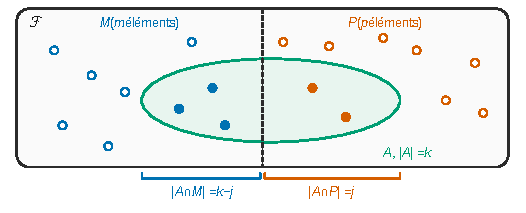
\includegraphics{figures/q09-vandermonde-double-comptage.pdf}
\caption*{Figure 1 --- Double comptage de Vandermonde : une partie A à k éléments
de ℱ = M ⊔ P se coupe en A ∩ M (k − j éléments) et A ∩ P (j éléments)}
\end{figure}

\hypertarget{q10}{%
\subsection{Q10}\label{q10}}

Si \(k=0\) : \(B^n_0=1=\binom n0\). Si \(1\leqslant k\leqslant n\) :

\equationajustee{\begin{aligned}B^n_k&=\frac{n(n-1)\cdots(n-k+1)}{k!}\\&=\frac{n!}{k!\,(n-k)!}\\&=\binom nk.\end{aligned}}

\textbf{Les deux nombres sont égaux : \(B^n_k=\binom nk\).}

\hypertarget{partie-c-une-famille-de-polynuxf4mes}{%
\section{Partie C --- Une famille de polynômes}\label{partie-c-une-famille-de-polynuxf4mes}}

\hypertarget{i-premiuxe8res-propriuxe9tuxe9s-des-p_k}{%
\subsection{\texorpdfstring{I -- Premières propriétés des \(P_k\)}{I -- Premières propriétés des P\_k}}\label{i-premiuxe8res-propriuxe9tuxe9s-des-p_k}}

\hypertarget{q11}{%
\subsection{Q11}\label{q11}}

D'après (i), \(P_k\in\mathrm{Vect}(P_0,\dots,P_k)=\mathbb R_k[X]\), donc \(\deg P_k\leqslant k\).

Pour \(k=0\), \(P_0\) est de norme \(1\), donc non nul : \(\deg P_0=0\).

Pour \(k\geqslant1\), supposons \(P_k\in\mathbb R_{k-1}[X]=\mathrm{Vect}(P_0,\dots,P_{k-1})\). Alors \(\mathbb R_k[X]=\mathrm{Vect}(P_0,\allowbreak \dots,\allowbreak P_k)\subset\mathbb R_{k-1}[X]\). Cela contredit \(\dim\mathbb R_k[X]=k+1>k\). \textbf{Donc \(\deg P_k=k\).}

\hypertarget{q12}{%
\subsection{Q12}\label{q12}}

Par (i), \(\mathrm{Vect}(1,\allowbreak \dots,\allowbreak X^{k-1})=\mathrm{Vect}(P_0,\allowbreak \dots,\allowbreak P_{k-1})\). La famille \(\mathcal B\) étant orthonormale, \(\langle P_k,P_j\rangle=0\) pour \(j\leqslant k-1\). Par linéarité, \(P_k\) est orthogonal à toute combinaison linéaire de \(P_0,\dots,P_{k-1}\) :

\equationajustee{\boxed{P_k\in\mathrm{Vect}(1,X,\dots,X^{k-1})^\perp.}}

\hypertarget{q13}{%
\subsection{Q13}\label{q13}}

Comme \(\deg Q=k\), on a \(Q\in\mathbb R_k[X]=\mathrm{Vect}(P_0,\dots,P_k)\). La base étant orthonormale :

\equationajustee{Q=\sum_{j=0}^k\langle Q,P_j\rangle P_j.}

Pour \(j\leqslant k-1\), \(P_j\in\mathbb R_{k-1}[X]\) (Q11). Comme \(Q\perp\mathbb R_{k-1}[X]\), on a \(\langle Q,P_j\rangle=0\).

Ainsi \(Q=\alpha_kP_k\) avec \(\alpha_k=\langle Q,P_k\rangle\) (non nul puisque \(Q\neq0\)).

\hypertarget{ii-une-relation-entre-p_k-1-p_k-et-p_k1}{%
\subsection{\texorpdfstring{II -- Une relation entre \(P_{k-1}\), \(P_k\) et \(P_{k+1}\)}{II -- Une relation entre P\_\{k-1\}, P\_k et P\_\{k+1\}}}\label{ii-une-relation-entre-p_k-1-p_k-et-p_k1}}

\hypertarget{q14}{%
\subsection{Q14}\label{q14}}

Notons \(\lambda_j\neq0\) le coefficient dominant de \(P_j\) (Q11).

Les polynômes \(P_{k+1}\) et \(XP_k\) sont de degré \(k+1\). Leurs coefficients dominants sont \(\lambda_{k+1}\) et \(\lambda_k\). Avec

\equationajustee{\boxed{a_k=\frac{\lambda_{k+1}}{\lambda_k},}}

le coefficient de \(X^{k+1}\) dans \(P_{k+1}-a_kXP_k\) est nul, donc \(\deg(P_{k+1}-a_kXP_k)\leqslant k\).

\hypertarget{q15}{%
\subsection{Q15}\label{q15}}

Soit \(R=P_{k+1}-a_kXP_k\in\mathbb R_k[X]\), donc \(R=\sum_{j=0}^k\langle R,P_j\rangle P_j\).

Pour tous \(A,B\in\mathbb R[X]\) :

\equationajustee{\begin{aligned}\langle XA,B\rangle&=\int_{-1}^1w(t)\,tA(t)B(t)\,dt\\&=\langle A,XB\rangle.\end{aligned}}

Pour \(j\in\{0,\dots,k-2\}\) (ensemble vide si \(k=1\)) :

\equationajustee{\begin{aligned}\langle R,P_j\rangle&=\langle P_{k+1},P_j\rangle-a_k\langle P_k,XP_j\rangle\\&=0-0\\&=0,\end{aligned}}

car \(j\neq k+1\) et \(XP_j\in\mathbb R_{k-1}[X]\) est orthogonal à \(P_k\) (Q12). Il reste \(R=b_kP_k+c_kP_{k-1}\), avec \(b_k=\langle R,P_k\rangle\) et \(c_k=\langle R,P_{k-1}\rangle\) :

\equationajustee{\boxed{P_{k+1}=(a_kX+b_k)P_k+c_kP_{k-1}.}}

La preuve n'utilise que l'orthogonalité et \(\deg P_j=j\). Elle vaut donc pour toute famille orthogonale échelonnée en degré, avec les coordonnées \(\langle R,P_j\rangle/\|P_j\|^2\).

\hypertarget{iii-racines-des-polynuxf4mes-p_k}{%
\subsection{\texorpdfstring{III -- Racines des polynômes \(P_k\)}{III -- Racines des polynômes P\_k}}\label{iii-racines-des-polynuxf4mes-p_k}}

\hypertarget{q16}{%
\subsection{Q16}\label{q16}}

\(P_k\) est non nul de degré \(k\) : il a au plus \(k\) racines comptées avec multiplicité. \textbf{Donc \(m\leqslant k\).}

\hypertarget{q17}{%
\subsection{Q17}\label{q17}}

Si \(\mathcal R=\varnothing\), \(P_kS=P_k\) est continue et ne s'annule pas sur l'intervalle \(]-1,1[\). Par le théorème des valeurs intermédiaires, elle y garde un signe strict constant.

Supposons \(m\geqslant1\). Le polynôme \(S\) regroupe les racines de \(P_k\) situées dans \(]-1,1[\), avec leurs multiplicités. Donc \(S\) divise \(P_k\).

Écrivons \(P_k=ST\), où \(T\) n'a aucune racine dans \(]-1,1[\). Par le théorème des valeurs intermédiaires, \(T\) garde un signe strict constant \(\varepsilon\) sur \(]-1,1[\). Alors

\equationajustee{P_kS=S^2T.}

\textbf{La fonction \(x\mapsto P_k(x)S(x)\) est de signe constant sur \(]-1,1[\)}, celui de \(T\). Elle ne s'y annule qu'en \(x_1,\dots,x_m\).

\begin{figure}[H]
\centering
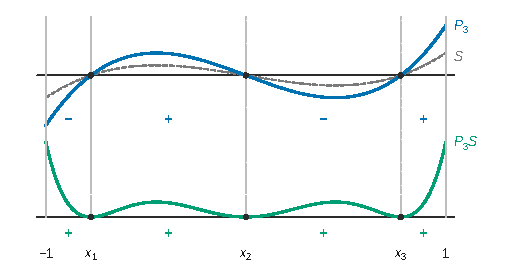
\includegraphics{figures/q17-signe-pk-s.pdf}
\caption*{Figure 2 --- Cas k = 3 : P₃ et S changent de signe aux mêmes racines x₁,
x₂, x₃ ; leur produit P₃S garde un signe constant (allure, échelles
verticales arbitraires)}
\end{figure}

\hypertarget{q18}{%
\subsection{Q18}\label{q18}}

La fonction \(\varphi=\varepsilon\,wP_kS\) est continue et positive sur \(]-1,1[\), et

\equationajustee{\varepsilon\langle P_k,S\rangle=\int_{-1}^1\varphi.}

Supposons cette intégrale nulle. L'argument de segment de Q4 donne \(\varphi=0\) sur \(]-1,1[\). Comme \(w>0\), on a \(P_kS=0\) sur cet intervalle.

Le polynôme \(P_kS\) a alors une infinité de racines : \(P_kS=0\). Comme \(S\neq0\), on obtient \(P_k=0\), ce qui contredit \(\deg P_k=k\). \textbf{Donc \(\langle P_k,S\rangle\neq0\).}

\hypertarget{q19}{%
\subsection{Q19}\label{q19}}

\(S\) est de degré \(m\). Si \(m\leqslant k-1\), alors \(S\in\mathbb R_{k-1}[X]\) et \(\langle P_k,S\rangle=0\) par Q12, ce qui contredit Q18. Donc \(m\geqslant k\) et, avec Q16 :

\equationajustee{\boxed{m=k.}}

\textbf{Toutes les racines de \(P_k\) sont réelles et situées dans \(]-1,1[\).}

Elles sont de plus simples. Soient \(y_1,\dots,y_r\) les racines de \(P_k\) dans \(]-1,1[\) de multiplicité impaire. Posons \(U=\prod(X-y_i)\).

Toutes les racines de \(P_kU\) dans cet intervalle sont de multiplicité paire.

Donc \(P_kU\) est de signe constant sur \(]-1,1[\), et non identiquement nulle. On en tire \(\langle P_k,U\rangle\neq0\), puis \(r\geqslant k\) ; donc \(P_k\) a \(k\) racines distinctes.

\hypertarget{partie-d-polynuxf4mes-de-jacobi}{%
\section{Partie D --- Polynômes de Jacobi}\label{partie-d-polynuxf4mes-de-jacobi}}

\hypertarget{i-duxe9finition}{%
\subsection{I -- Définition}\label{i-duxe9finition}}

\hypertarget{q20}{%
\subsection{Q20}\label{q20}}

On a \(g_0(x)=(1-x)^\alpha(1+x)^\beta\) et \(g_1(x)=(1-x)^{\alpha+1}(1+x)^{\beta+1}\). Donc \(J_0=1\). Puis

\equationajustee{\begin{aligned}g_1'(x)&=(1-x)^\alpha(1+x)^\beta\big[-(\alpha+1)(1+x)+(\beta+1)(1-x)\big]\\&=(1-x)^\alpha(1+x)^\beta\big[(\beta-\alpha)-(\alpha+\beta+2)x\big],\end{aligned}}

et \(J_1=-\dfrac{g_1'}{2(1-x)^\alpha(1+x)^\beta}\) :

\equationajustee{\boxed{\begin{aligned}J_0&=1\\J_1&=\frac{(\alpha+\beta+2)X+\alpha-\beta}{2}\end{aligned}}}

\hypertarget{q21}{%
\subsection{Q21}\label{q21}}

Montrons par récurrence sur \(p\) que, sur \(]-1,1[\) :

\equationajustee{\frac{d^p}{dx^p}(1-x)^j=(-1)^p\,p!\,B^j_p\,(1-x)^{j-p}.}

C'est vrai pour \(p=0\). Si c'est vrai au rang \(p\), en dérivant :

\equationajustee{\begin{aligned}\frac{d^{p+1}}{dx^{p+1}}(1-x)^j&=(-1)^p\,p!\,B^j_p\,(j-p)(-1)(1-x)^{j-p-1}\\&=(-1)^{p+1}(p+1)!\,B^j_{p+1}(1-x)^{j-p-1},\end{aligned}}

car \((p+1)!\,B^j_{p+1}=j(j-1)\cdots(j-p)\), qui vaut \(p!\,B^j_p\,(j-p)\) (valable aussi pour \(p=0\)). D'où

\equationajustee{\boxed{\frac{d^p}{dx^p}(1-x)^j=(-1)^p\,p!\,B^j_p\,(1-x)^{j-p}.}}

De même, \(\dfrac{d^p}{dx^p}(1+x)^j=p!\,B^j_p\,(1+x)^{j-p}\).

\hypertarget{q22}{%
\subsection{Q22}\label{q22}}

Par la formule de Leibniz et Q21, pour \(p\in\{0,\dots,k\}\) :

\equationajustee{g_k^{(p)}(x)=\sum_{i=0}^p\binom pi(-1)^ii!\,B^{\alpha+k}_i(1-x)^{\alpha+k-i}\,(p-i)!\,B^{\beta+k}_{p-i}(1+x)^{\beta+k-p+i}.}

Avec \(\binom pi i!(p-i)!=p!\), on obtient

\equationajustee{g_k^{(p)}(x)=(1-x)^{\alpha+k-p}(1+x)^{\beta+k-p}\,h_p(x),}

où

\equationajustee{h_p(x)=p!\sum_{i=0}^p(-1)^iB^{\alpha+k}_iB^{\beta+k}_{p-i}(1-x)^{p-i}(1+x)^i}

est polynomiale de degré au plus \(p\). En particulier :

\equationajustee{\boxed{g_k^{(k)}(x)=k!\,(1-x)^\alpha(1+x)^\beta\sum_{i=0}^k(-1)^iB^{\alpha+k}_iB^{\beta+k}_{k-i}(1-x)^{k-i}(1+x)^i.}}

\hypertarget{q23}{%
\subsection{Q23}\label{q23}}

En reportant dans la définition de \(J_k\), le poids et \(k!\) se simplifient :

\equationajustee{J_k(x)=\frac1{2^k}\sum_{i=0}^k(-1)^{k+i}B^{\alpha+k}_iB^{\beta+k}_{k-i}(1-x)^{k-i}(1+x)^i.}

Comme \((-1)^{k+i}=(-1)^{k-i}\), on a \((-1)^{k+i}(1-x)^{k-i}=(x-1)^{k-i}\). Le changement d'indice \(i\mapsto k-i\) donne

\equationajustee{\boxed{J_k(x)=\frac1{2^k}\sum_{i=0}^kB^{k+\alpha}_{k-i}B^{k+\beta}_i(x-1)^i(x+1)^{k-i}.}}

(Le calcul vaut pour tout \(k\geqslant0\).)

\hypertarget{q24}{%
\subsection{Q24}\label{q24}}

Chaque \((x-1)^i(x+1)^{k-i}\) est polynomial, de degré \(k\) et unitaire. Donc \(J_k\) coïncide sur \(]-1,1[\) avec un polynôme de degré au plus \(k\). Son coefficient de \(X^k\) est

\equationajustee{\lambda_k=\frac1{2^k}\sum_{i=0}^kB^{k+\alpha}_{k-i}B^{k+\beta}_i.}

Pour \(k\geqslant2\), on a \(k\leqslant2k+\alpha+\beta\) (car \(\alpha+\beta>-2\)). La formule de Vandermonde généralisée, avec \(s=k+\alpha\) et \(t=k+\beta\), donne

\equationajustee{\boxed{\begin{aligned}\lambda_k&=\frac{B^{2k+\alpha+\beta}_k}{2^k}\\&=\frac1{2^kk!}\prod_{r=0}^{k-1}(2k+\alpha+\beta-r).\end{aligned}}}

Chaque facteur vérifie

\equationajustee{2k+\alpha+\beta-r\geqslant k+1+\alpha+\beta>k-1>0,}

donc \(\lambda_k>0\) : \textbf{\(J_k\) est polynomiale de degré exactement \(k\).}

Pour \(k=0\) et \(k=1\), Q20 donne directement les valeurs suivantes, que la formule encadrée redonne :

\equationajustee{\begin{aligned}\lambda_0&=1,\\\lambda_1&=\frac{\alpha+\beta+2}2>0.\end{aligned}}

\hypertarget{ii-orthogonalituxe9-des-polynuxf4mes-de-jacobi}{%
\subsection{II -- Orthogonalité des polynômes de Jacobi}\label{ii-orthogonalituxe9-des-polynuxf4mes-de-jacobi}}

\hypertarget{q25}{%
\subsection{Q25}\label{q25}}

\emph{Convergence.} Par Q22 :

\equationajustee{\begin{aligned}x^ig_k^{(k)}(x)&=(1-x)^\alpha(1+x)^\beta\,x^ih_k(x),\\x^{i-1}g_k^{(k-1)}(x)&=(1-x)^{\alpha+1}(1+x)^{\beta+1}\,x^{i-1}h_{k-1}(x).\end{aligned}}

La fonction \(x^ih_k\) est continue sur \([-1,1]\). Pour \(i\geqslant1\), il en va de même de \(x^{i-1}h_{k-1}\). Les exposants \(\alpha,\beta,\alpha+1,\beta+1\) sont \(>-1\). Q3 donne donc la convergence des deux intégrales.

\emph{Intégration par parties} sur \([u,v]\subset]-1,1[\) :

\equationajustee{\int_u^vx^ig_k^{(k)}=\Big[x^ig_k^{(k-1)}(x)\Big]_u^v-i\int_u^vx^{i-1}g_k^{(k-1)}.}

\emph{Termes de bord} : on a la majoration

\equationajustee{|x^ig_k^{(k-1)}(x)|\leqslant\|h_{k-1}\|_\infty(1-x)^{\alpha+1}(1+x)^{\beta+1},}

dont le second membre tend vers \(0\) en \(\pm1\). En effet, \(\alpha+1>0\) et \(\beta+1>0\).

En faisant \(u\to-1\) et \(v\to1\) :

\equationajustee{\boxed{\int_{-1}^1x^ig_k^{(k)}(x)\,dx=-i\int_{-1}^1x^{i-1}g_k^{(k-1)}(x)\,dx.}}

Pour \(i=0\), la seconde intégrale n'a pas de sens en général : pour \(k=1\), l'intégrande est équivalent à \(1/x\) en \(0\). L'identité se lit alors \(\int_{-1}^1g_k^{(k)}=0\), ce que donne le même calcul :

\equationajustee{\begin{aligned}\int_{-1}^1g_k^{(k)}&=\big[g_k^{(k-1)}\big]_{-1}^1\\&=0.\end{aligned}}

\hypertarget{q26}{%
\subsection{Q26}\label{q26}}

Par définition de \(J_k\), \(w(t)J_k(t)t^i=\dfrac{(-1)^k}{2^kk!}t^ig_k^{(k)}(t)\), donc

\equationajustee{\langle J_k,X^i\rangle=\dfrac{(-1)^k}{2^kk!}\displaystyle\int_{-1}^1t^ig_k^{(k)}.}

Le raisonnement de Q25 s'applique à tout ordre \(p\in\{1,\dots,k\}\). En effet, par Q22 :

\equationajustee{g_k^{(p-1)}=(1-x)^{\alpha+k-p+1}(1+x)^{\beta+k-p+1}h_{p-1},}

avec des exposants \(\geqslant\alpha+1>0\) et \(\geqslant\beta+1>0\). D'où, pour \(j\geqslant1\) :

\equationajustee{\int_{-1}^1x^jg_k^{(p)}=-j\int_{-1}^1x^{j-1}g_k^{(p-1)}.}

On l'applique \(i\) fois, aux ordres \(k,k-1,\dots,k-i+1\), tous \(\geqslant1\) :

\equationajustee{\begin{aligned}\int_{-1}^1x^ig_k^{(k)}&=(-1)^ii!\int_{-1}^1g_k^{(k-i)}\\&=(-1)^ii!\Big[g_k^{(k-i-1)}\Big]_{-1}^1\\&=0,\end{aligned}}

car \(k-i-1\geqslant0\), et \(g_k^{(k-i-1)}\) tend vers \(0\) aux deux bornes. Ses exposants sont en effet \(\alpha+i+1>0\) et \(\beta+i+1>0\).

\textbf{Donc \(\langle J_k,X^i\rangle=0\).}

\hypertarget{q27}{%
\subsection{Q27}\label{q27}}

Les \(J_k\) sont non nuls et de degrés \(0,1,\dots,n\) deux à deux distincts (Q24) : la famille est libre. Elle compte \(n+1=\dim E\) vecteurs : c'est une base de \(E\).

Pour \(i<k\), \(J_i\in\mathbb R_{k-1}[X]\) est combinaison linéaire de \(1,\dots,X^{k-1}\). Donc \(\langle J_k,J_i\rangle=0\) par Q26. \textbf{\((J_0,\dots,J_n)\) est une base orthogonale de \(E\).}

\hypertarget{q28}{%
\subsection{Q28}\label{q28}}

Chaque \(J_k\) est non nul, donc \(\|J_k\|>0\). La famille \(\Big(\dfrac{J_k}{\|J_k\|}\Big)_{0\leqslant k\leqslant n}\) est orthogonale, formée de vecteurs unitaires : \textbf{c'est une base orthonormale de \(E\).}

C'est même la base \(\mathcal B\) de la partie C. En effet, \(J_k/\|J_k\|\) est de degré \(k\) et orthogonal à \(\mathbb R_{k-1}[X]\). Il vaut donc \(\pm P_k\) par Q13.

Écrivons \(X^k=J_k/\lambda_k+\) termes de degré \(<k\). On obtient

\equationajustee{\langle J_k,X^k\rangle=\frac{\|J_k\|^2}{\lambda_k}>0,}

ce qui fixe le signe \(+\) par (ii).

\hypertarget{partie-e-le-cas-particulier-alphabeta00}{%
\section{\texorpdfstring{Partie E --- Le cas particulier \((\alpha,\beta)=(0,0)\)}{Partie E --- Le cas particulier (\textbackslash alpha,\textbackslash beta)=(0,0)}}\label{partie-e-le-cas-particulier-alphabeta00}}

Pour \(\alpha=\beta=0\), on a \(g_k=(1-x^2)^k=(-1)^k(x^2-1)^k\), d'où

\equationajustee{\begin{aligned}J_k&=\frac{1}{2^kk!}\big[(X^2-1)^k\big]^{(k)}\\&=L_k.\end{aligned}}

Les \(L_k\) sont les \(J_k\), orthogonaux mais non normés (\(\|L_0\|^2=2\)). Les résultats de Q14--Q15 restent valables pour eux (remarque de Q15).

\hypertarget{i-premiuxe8res-propriuxe9tuxe9s-des-polynuxf4mes-l_k}{%
\subsection{\texorpdfstring{I -- Premières propriétés des polynômes \(L_k\)}{I -- Premières propriétés des polynômes L\_k}}\label{i-premiuxe8res-propriuxe9tuxe9s-des-polynuxf4mes-l_k}}

\hypertarget{q29}{%
\subsection{Q29}\label{q29}}

On a \((X^2-1)^2=X^4-2X^2+1\), de dérivée seconde \(12X^2-4\).

De même, \((X^2-1)^3=X^6-3X^4+3X^2-1\), de dérivée troisième \(120X^3-72X\). D'où

\equationajustee{\boxed{\begin{aligned}L_0&=1\\L_1&=X\\L_2&=\frac{3X^2-1}2\\L_3&=\frac{5X^3-3X}2\end{aligned}}}

\hypertarget{q30}{%
\subsection{Q30}\label{q30}}

\(L_1\) : racine \(0\).

\(L_2\) : racines \(\pm\frac1{\sqrt3}\approx\pm0{,}577\).

\(L_3=\frac{X(5X^2-3)}2\) : racines \(0\) et \(\pm\sqrt{\frac35}\approx\pm0{,}775\).

Dans chaque cas, les \(k\) racines sont réelles, simples et dans \(]-1,1[\) : \textbf{\(m=k\), conformément à Q19.}

\begin{figure}[H]
\centering
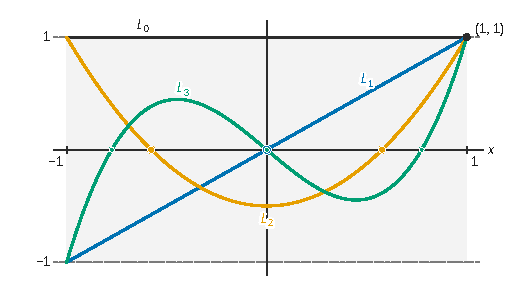
\includegraphics{figures/q30-polynomes-legendre.pdf}
\caption*{Figure 3 --- Polynômes de Legendre L₀ à L₃ entre −1 et 1 : L\_k a k
racines simples, vaut 1 en x = 1 et reste dans la bande
\textbar y\textbar{} ⩽ 1}
\end{figure}

\hypertarget{q31}{%
\subsection{Q31}\label{q31}}

On a \((X^2-1)^k=X^{2k}+(\text{termes de \text{degré}}<2k)\).

La dérivée \(k\)-ième de \(X^{2k}\) est \(\frac{(2k)!}{k!}X^k\). Celle d'un monôme de degré \(r<2k\) est de degré \(<k\) (ou nulle). Donc \(\deg L_k=k\) et

\equationajustee{\boxed{\begin{aligned}\text{coefficient dominant de }L_k&=\frac{(2k)!}{2^k(k!)^2}\\&=\frac1{2^k}\binom{2k}k.\end{aligned}}}

(On retrouve \(B^{2k}_k/2^k\) de Q24, par Q10.)

\hypertarget{q32}{%
\subsection{Q32}\label{q32}}

Soit \(Q\) pair. En dérivant \(Q^{(p)}(-x)=(-1)^pQ^{(p)}(x)\), une récurrence donne cette relation pour tout \(p\). Avec \(Q=(X^2-1)^k\) et \(p=k\) :

\equationajustee{\boxed{L_k(-X)=(-1)^kL_k(X)}}

\textbf{\(L_k\) a la parité de \(k\).}

\hypertarget{q33}{%
\subsection{Q33}\label{q33}}

La formule de Leibniz appliquée à \((X-1)^k(X+1)^k\) donne

\equationajustee{\big[(X^2-1)^k\big]^{(k)}=\sum_{i=0}^k\binom ki\big[(X-1)^k\big]^{(i)}\big[(X+1)^k\big]^{(k-i)}.}

En \(x=1\), seul subsiste le terme \(i=k\) : les autres contiennent \((x-1)^{k-i}\), avec \(k-i\geqslant1\). Ce terme vaut \(k!\,2^k\). Avec Q32 :

\equationajustee{\boxed{\begin{aligned}L_k(1)&=1\\L_k(-1)&=(-1)^k\end{aligned}}}

\hypertarget{ii-une-uxe9quation-diffuxe9rentielle-vuxe9rifiuxe9e-par-les-l_k}{%
\subsection{\texorpdfstring{II -- Une équation différentielle vérifiée par les \(L_k\)}{II -- Une équation différentielle vérifiée par les L\_k}}\label{ii-une-uxe9quation-diffuxe9rentielle-vuxe9rifiuxe9e-par-les-l_k}}

\hypertarget{q34}{%
\subsection{Q34}\label{q34}}

Pour \(k\geqslant1\), \(g_k'(x)=-2kx(1-x^2)^{k-1}\) ; pour \(k=0\), \(g_0'=0\). Dans tous les cas :

\equationajustee{\boxed{(1-x^2)g_k'(x)=-2kx\,g_k(x).}}

\hypertarget{q35}{%
\subsection{Q35}\label{q35}}

Notons \(u=g_k\). Dérivons \(k+1\) fois \((1-x^2)u'+2kxu=0\) par Leibniz.

Les dérivées de \(1-x^2\) sont nulles à partir de l'ordre 3, celles de \(x\) à partir de l'ordre 2 :

\equationajustee{(1-x^2)u^{(k+2)}-2(k+1)xu^{(k+1)}-k(k+1)u^{(k)}+2k\big(xu^{(k+1)}+(k+1)u^{(k)}\big)=0,}

soit

\equationajustee{(1-x^2)\big(u^{(k)}\big)''-2x\big(u^{(k)}\big)'+k(k+1)u^{(k)}=0.}

Comme \(u^{(k)}=(-1)^k2^kk!\,L_k\), on divise par cette constante non nulle :

\equationajustee{\boxed{(1-x^2)L_k''-2xL_k'+k(k+1)L_k=0\ \text{ sur }]-1,1[.}}

\hypertarget{iii-une-majoration-des-l_k-sur--11}{%
\subsection{\texorpdfstring{III -- Une majoration des \(L_k\) sur \([-1,1]\)}{III -- Une majoration des L\_k sur {[}-1,1{]}}}\label{iii-une-majoration-des-l_k-sur--11}}

\hypertarget{q36}{%
\subsection{Q36}\label{q36}}

\(f_k\) n'est définie que pour \(k\geqslant1\). Alors

\equationajustee{f_k'=2L_kL_k'+\frac{2L_k'}{k(k+1)}\big[(1-x^2)L_k''-xL_k'\big].}

L'équation de Q35, identité polynomiale vraie sur \(]-1,1[\), est vraie sur \(\mathbb R\). Elle donne

\equationajustee{(1-x^2)L_k''-xL_k'=xL_k'-k(k+1)L_k.}

D'où

\equationajustee{\boxed{f_k'(x)=\frac{2x}{k(k+1)}L_k'(x)^2\geqslant0\ \text{ sur }[0,1]}}

\textbf{\(f_k\) est croissante sur \([0,1]\).}

\hypertarget{q37}{%
\subsection{Q37}\label{q37}}

Pour \(k=0\), \(L_0=1\). Pour \(k\geqslant1\) et \(x\in[0,1]\), comme \(1-x^2\geqslant0\) :

\equationajustee{\begin{aligned}L_k(x)^2&\leqslant f_k(x)\\&\leqslant f_k(1)\\&=L_k(1)^2\\&=1\end{aligned}}

(Q36 puis Q33). Pour \(x\in[-1,0]\), \(|L_k(x)|=|L_k(-x)|\leqslant1\) par Q32. \textbf{Donc \(|L_k(x)|\leqslant1\) sur \([-1,1]\).}

\hypertarget{iv-relation-entre-l_k-1-l_k-et-l_k1}{%
\subsection{\texorpdfstring{IV -- Relation entre \(L_{k-1}\), \(L_k\) et \(L_{k+1}\)}{IV -- Relation entre L\_\{k-1\}, L\_k et L\_\{k+1\}}}\label{iv-relation-entre-l_k-1-l_k-et-l_k1}}

\hypertarget{q38}{%
\subsection{Q38}\label{q38}}

Pour la famille orthogonale échelonnée \((L_j)\), \(a_k\) est le quotient des coefficients dominants (Q14, Q31) :

\equationajustee{\begin{aligned}a_k&=\frac{(2k+2)!}{2^{k+1}((k+1)!)^2}\cdot\frac{2^k(k!)^2}{(2k)!}\\&=\frac{(2k+2)(2k+1)}{2(k+1)^2},\end{aligned}}

\equationajustee{\boxed{a_k=\frac{2k+1}{k+1}.}}

\hypertarget{q39}{%
\subsection{Q39}\label{q39}}

Par Q15 (valable pour la famille orthogonale \((L_j)\)) :

\equationajustee{L_{k+1}=(a_kX+b_k)L_k+c_kL_{k-1}.}

\emph{\(b_k=0\)} : par Q32, les polynômes \(L_{k+1}\), \(XL_k\) et \(L_{k-1}\) ont tous la parité de \(k+1\).

Donc \(b_kL_k=L_{k+1}-a_kXL_k-c_kL_{k-1}\) a la parité de \(k+1\) et celle de \(k\). Il est donc nul, et \(L_k\neq0\) impose \(b_k=0\).

\emph{\(c_k\)} : en \(x=1\), Q33 donne \(1=a_k+c_k\), soit

\equationajustee{\begin{aligned}c_k&=1-\frac{2k+1}{k+1}\\&=-\frac k{k+1}.\end{aligned}}

\equationajustee{\boxed{L_{k+1}=\frac{2k+1}{k+1}XL_k-\frac k{k+1}L_{k-1}.}}

\hypertarget{v-un-duxe9veloppement-en-suxe9rie-entiuxe8re-faisant-intervenir-les-l_k}{%
\subsection{\texorpdfstring{V -- Un développement en série entière faisant intervenir les \(L_k\)}{V -- Un développement en série entière faisant intervenir les L\_k}}\label{v-un-duxe9veloppement-en-suxe9rie-entiuxe8re-faisant-intervenir-les-l_k}}

\hypertarget{q40}{%
\subsection{Q40}\label{q40}}

Par Q37, \(|L_k(x)|\leqslant1\) pour tout \(k\). Soit \(r\in[0,1[\) : la suite \((L_k(x)r^k)\) est bornée.

Le rayon \(R_x\) vérifie donc \(R_x\geqslant r\). Ceci vaut pour tout \(r<1\) :

\equationajustee{\boxed{R_x\geqslant1.}}

\hypertarget{q41}{%
\subsection{Q41}\label{q41}}

Sur \(]-1,1[\), \(S\) est dérivable terme à terme :

\equationajustee{S'(t)=\sum_{k\geqslant0}(k+1)L_{k+1}(x)t^k.}

On utilise la relation suivante, vraie pour \(k\geqslant1\) par Q39, et pour \(k=0\) car \(L_1=xL_0\) :

\equationajustee{(k+1)L_{k+1}=(2k+1)xL_k-kL_{k-1}.}

Toutes les séries ci-dessous ont un rayon \(\geqslant1\) :

\equationajustee{\begin{aligned}S'(t)&=2x\sum_{k\geqslant0}kL_kt^k+x\sum_{k\geqslant0}L_kt^k-\sum_{k\geqslant1}kL_{k-1}t^k\\&=2xtS'(t)+xS(t)-t\big(tS'(t)+S(t)\big),\end{aligned}}

car

\equationajustee{\begin{aligned}\sum_{k\geqslant1}kL_{k-1}t^k&=\sum_{j\geqslant0}(j+1)L_jt^{j+1}\\&=t\big(tS'+S\big).\end{aligned}}

En regroupant :

\equationajustee{\boxed{(1-2tx+t^2)S'(t)+(t-x)S(t)=0.}}

\hypertarget{q42}{%
\subsection{Q42}\label{q42}}

Soit \(\varphi(t)=1-2tx+t^2\). On a

\equationajustee{\varphi(t)=(t-x)^2+1-x^2.}

Si \(|x|<1\), \(\varphi>0\). Si \(x=\pm1\), \(\varphi(t)=(t\mp1)^2>0\) pour \(t\in]-1,1[\).

Ainsi \(\varphi>0\) sur \(]-1,1[\), avec \(\varphi'(t)=2(t-x)\).

Posons \(H=S\sqrt\varphi\). Alors

\equationajustee{\begin{aligned}H'&=S'\sqrt\varphi+S\frac{\varphi'}{2\sqrt\varphi}\\&=\frac{\varphi S'+(t-x)S}{\sqrt\varphi}\\&=0\end{aligned}}

par Q41. Donc \(H\) est constante sur l'intervalle \(]-1,1[\), égale à \(H(0)=S(0)=L_0(x)=1\). Donc, pour tout \(t\in]-1,1[\) :

\equationajustee{\boxed{\sum_{k=0}^{+\infty}L_k(x)t^k=\frac1{\sqrt{1-2tx+t^2}}.}}

\end{document}
